\documentclass{article}
\usepackage[margin=30mm]{geometry}
\usepackage{graphicx}
\begin{document}
\title{1506801 Submission 2}
\author{Jack Neilson}
\maketitle
\newpage
\section*{Activity 3}
\obeylines
\subsection*{A}

female(tuya).
female(tiy).
female(unknown).
female(kiya).
female(nefertiti).
female(ankhesenamun).
female(other1).
female(other2).
female(other3).
female(other4).
female(merytaten).
female(stillborn1).
female(stillborn2).

male(yuya).
male(amenhotepiii).
male(ay).
male(akhenaten).
male(tutankhamun).
male(smenkhkare).

parent(tutankhamun, stillborn1).
parent(tutankhamun, stillborn2).
parent(ankhesenamun, stillborn1).
parent(ankhesenamun, stillborn2).

parent(kiya, tutankhamun).

parent(akhenaten, tutankhamun).
parent(akhenaten, ankhesenamun).
parent(akhenaten, other1).
parent(akhenaten, other2).
parent(akhenaten, other3).
parent(akhenaten, other4).
parent(akhenaten, merytaten).

parent(nefertiti, ankhesenamun).
parent(nefertiti, other1).
parent(nefertiti, other2).
parent(nefertiti, other3).
parent(nefertiti, other4).
parent(nefertiti, merytaten).

parent(amenhotepiii, akhenaten).

parent(tiy, akhenaten).

parent(ay, nefertiti).

parent(unknown, nefertiti).

parent(tuya, tiy).
parent(tuya, ay).

parent(yuya, tiy).
parent(yuya, ay).


partner(tuya, yuya).
partner(yuya, tuya).
partner(amenhotepiii,tiy).
partner(tiy,amenhotepiii).
partner(ay,unknown).
partner(unknown,ay).
partner(kiya, akhenaten).
partner(akhenaten, kiya).
partner(akhenaten, nefertiti).
partner(nefertiti, akhenaten).
partner(tutankhamun, ankhesenamun).
partner(ankhesenamun, tutankhamun).
partner(merytaten, smenkhkare).
partner(smenkhkare, merytaten).

\newpage
\subsection*{B}

\%Parent and partner already part of facts set.

mother(M,X) :- parent(M,X), female(M).

father(F,X) :- parent(F,X), male(F).

sibling(X,Y) :- parent(A,X), parent(A,Y), not(X = Y).

sister(W,Z) :- sibling(W,Z), female(W).

aunt(W,Z) :- parent(A,Z), sibling(W,A), female(W).

grandfather(W,Z) :- parent(A,Z), father(W,A).

ancestor(W,Z) :- parent(W,Z).
ancestor(W,Z) :- parent(W,A), ancestor(A,Z).

nephew(W,Z) :- parent(W,A), sibling(A,Z), male(W).

\newpage
\subsection*{C}

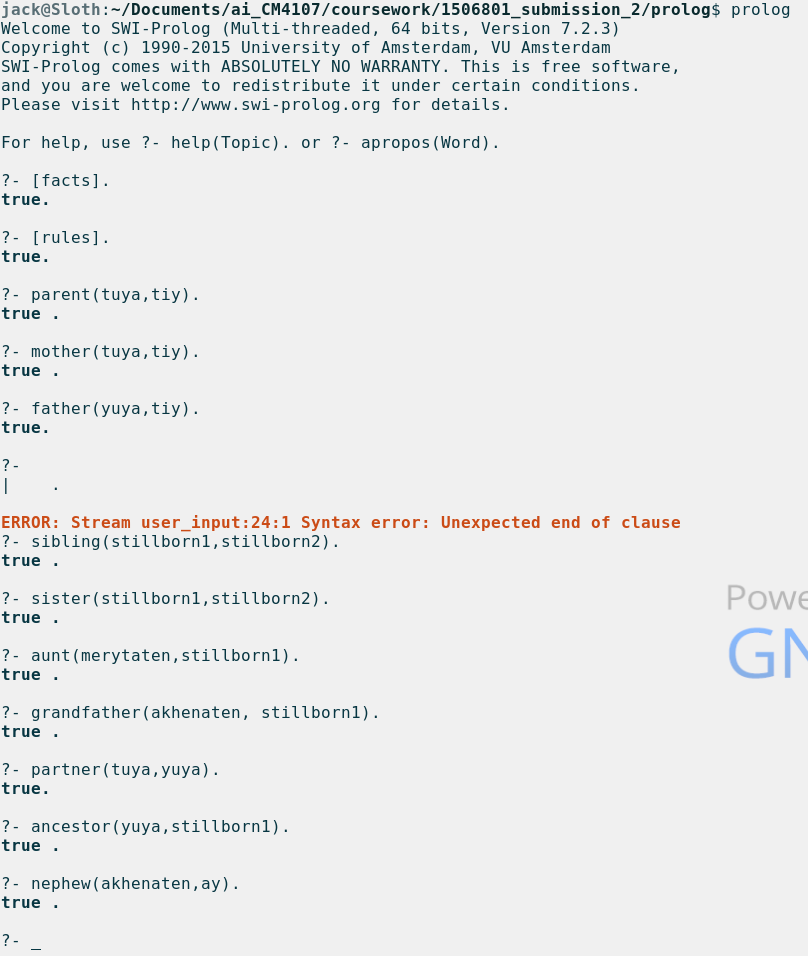
\includegraphics[scale=0.5]{testing}

\newpage
\section*{Activity 4}
\subsection*{A}
\subsubsection*{Data Structures}
Both the input and output pattern can be stored as arrays of integers which are analogous to the vectors used in the paper, the synaptic matrix can be represented as a two-dimensional array of integers.

The algorithm for comparing the input pattern to the synaptic matrix will be the same as the one used in the paper, i.e. a neuron should fire if the recall function (r = input * matrix) is greater than or equal to the sum of the input.

input = {1, 0, 0, 1};
inputSum = 0;
outputSum = {0, 0, 0, 0};
synapticMatrix = {{1, 0, 0, 1}, {0, 1, 0, 0}, {0, 0, 0, 0}, {1, 0, 0, 1}};

for (i = 0; i < input.length; i++) {
	inputSum += input[i];
}

for (i = 0; i < 

\end{document}
